%!TEX root = ../TAMUTemplate.tex
%%%%%%%%%%%%%%%%%%%%%%%%%%%%%%%%%%%%%%%%%%%%%%%%%%%
%
%  New template code for TAMU Theses and Dissertations starting Fall 2016.
%
%  Author: Sean Zachary Roberson
%	 Version 3.16.09
%  Last updated 9/12/2016
%
%%%%%%%%%%%%%%%%%%%%%%%%%%%%%%%%%%%%%%%%%%%%%%%%%%%
%%%%%%%%%%%%%%%%%%%%%%%%%%%%%%%%%%%%%%%%%%%%%%%%%%%%%%%%%%%%%%%%%%%%%%
%%                           SECTION IV
%%%%%%%%%%%%%%%%%%%%%%%%%%%%%%%%%%%%%%%%%%%%%%%%%%%%%%%%%%%%%%%%%%%%%



\chapter{\uppercase {Event Reconstruction}}
\label{ch:event_reconstruction}

The CMS detector is designed to identify the various particle species which travel through it after a proton-proton collision.
As discussed in chapter~\ref{ch:LHC_CMS}, the sub-detector technologies were chosen so that particles could be identified by where they deposite their energy as well as how their trajectories change in a magnetic field.
Fig~\ref{fig:particle_flow} shows how various types of particles interact with the CMS detector.
All of the charged particles (\ie electrons, muons, and charged hadrons) will deposit some energy in the tracker, while neutral particles (\ie photons and neutral hadrons) will not.
Electrons and photons will deposit all of their energy inside of the ECAL while hadrons, both charged and neutral, will deposit most of their energy in the HCAL.
Muons are the only visible particle which will be able to travel to the muon chambers.
Neutrinos will pass through all layers of the detector unseen and their presence must be infered by missing transverse energy (\MET or \ETslash); the idea being that if the sum of the transverse momentum is not conserved, then that missing momentum must correspond to at least one unseen particle.

\begin{figure}[!hbt]
	\centering
	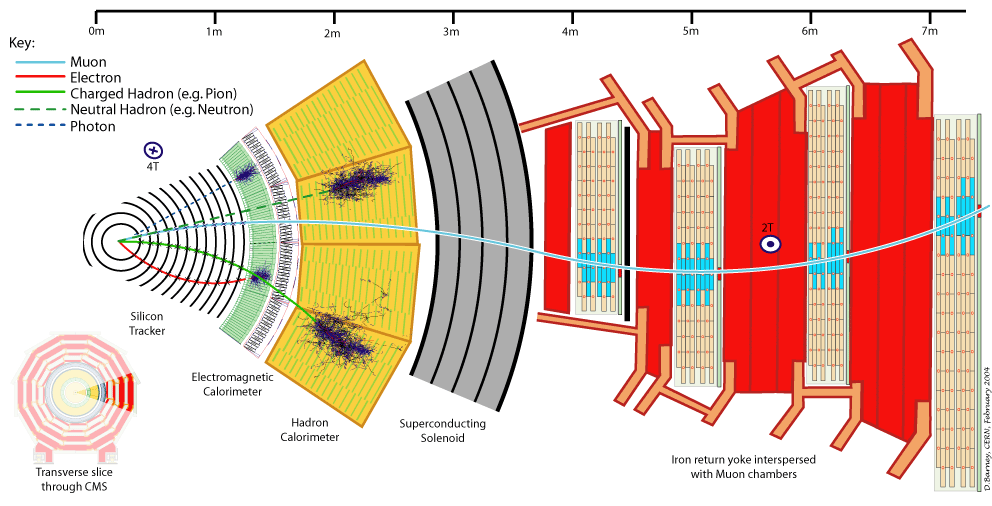
\includegraphics[width=0.95\textwidth]{\figpath/Chapter3/ParticleFlow}
	\caption{Cross-sectional view of the CMS detector with all of the sub-detectors labeled.The colored lines correspond to different particle species, which interact with different pieces of the detector and may or may not be bent by the magnetic field.}
	\label{fig:particle_flow}
\end{figure}

The process of translating abstract detector objects to physical particles takes several steps within the CMS software framework (CMSSW).
The first of this process is local reconstruction, where the various subsystems of each sub-detector create what are called reconstucted hits, or RecHits for short.
RecHits in the tracker contain information about the position of energy clusters (groups of contiguous strips or pixels which contain a signal) as well as energy deposition information which aids in particle identification.
The muon RecHits ostensibly contain information about the position of the signal.
However, the RecHits from the DTs and CSCs can be combined to form three-dimensional track segments, which also provide directional information.
The ECAL and HCAL RecHits contain information about the energy deposited, the position of those deposits, and the time at which they occured.

The next step is to process this information in a global manner, where the subsystems within each sub-detector are combined.
Pattern recongnition algorithms are run on the tracker RecHits to reconstruct the path that the particles take through the sub-detector (a.k.a tracks).
The ECAL and HCAL RecHits within a tower are summed to form ``CaloTowers'' which have a projective $\eta-\varphi$ geometry.
The muon system creates ``standalone'' muons by associating RecHits and track segments with compatible radial trajectories.
This process takes into account the bending a muon undergoes before reaching and within the muon system due to the magnetic field.

At this point, all of the reconstuction information is combined to form particles that can be used for physics analysis.
The process of reconstucting and classifying every stable particle is called Particle Flow (PF) and will be discussed further in chapter~\ref{sec:particle_flow}.
This analysis focuses on electrons, muons, jets, b-jets, and \ETslash, the reconstuction of which will be described in the following sections.
Additional information about the reconstruction process beyond the scope of this thesis can be found in~\cite{TDR-software}.

\section{Tracks and Vetices}
\label{sec:tracks_and_vertices}

While CMS analyses cover a wide range of final states, a majority of them will include jets in some fashion, including this one.
It's important that the particle flow algorithm identify and measure each particle inside a jet in order to improve the jet energy response and resolution.
Section~\ref{sec:jets} will cover the reconstruction and properties of jets in more detail, but it is important to note that two thirds of the constituents inside of a jet are charged particles.
This motivates the need for excellent tracking capabilities.
Tracks are created from the RecHits using the Combinatorial Track Finder (CTF) algorithm, which is an iterative process~\cite{TRK-11-001}.
This process seeks to find the appropriate balance between high reconstruction efficiency and low fake rate (see fig~\ref{fig:efficiency_vs_fake_rate})~\cite{CMS-PAS-PFT-09-001}.

\begin{figure}[!hbt]
	\centering
	\begin{tikzpicture}[node distance = 2cm, auto]
		\tikzstyle{myarrows}=[line width=1mm,-triangle 45,postaction={draw, line width=3mm, shorten >=4mm, -}]
	
		\node (up) at (0,2) {};
		\node (center) at (0,0) {};
		\node (down) at (0,-2) {};
	
		\draw[myarrows,green!50!black] (center) -- node[right,black,xshift=5mm] {Reconstruction Efficiency} ++ (up);
		\draw[myarrows,red] (center) -- node[right,black,xshift=5mm] {Fake Rate} ++ (down);
	
		\node (smiley) at (-1,1)  {\Smiley[3][green!50!black]};
		\node (sadey)  at (-1,-1) {\Sadey[3][red]};
	\end{tikzpicture}
	\caption{A diagram showing the goals of the iterative tracking process.}
	\label{fig:efficiency_vs_fake_rate}
\end{figure}

The track finding proceedure begins by finding track seeds using only a few hits and very tight criteria.
A track is built by extrpolating from the trajectory of the seed and adding new hits that match this trajectory, keeping in mind that charged particles will bend in the presence of the magnetic field.
The tight requirements on this first step lead to a moderate tracking efficiency and a vanishingly small fake rate.
After a track is found, all of the hits are used in a fit to determine the track parameters (i.e. \pt, $\chi^{2}$, etc.), which are then used to judge the quality of the track.
If a track doesn't meet certain quality requirments on the \pt, the transverse impact parameter $d_{0}$, and the longitudinal impact parameter $z_{0}$, it isn't kept.
Additionally, a trajectory cleaning step to remove duplicate tracks is applied to each iteration and to the final track collection.
A duplicate track can form either from different seeds or from the same seed which forms two very similar tracks.
If a pair of any two tracks share more than 19\% of hits as determined by equation~\ref{eq:trajectory_cleaning}, where $N^{hits}_{1}$ and $N^{hits}_{2}$ are the number of hits used in forming the tracks and 19\% is an empirically determined value, then the track with the fewest number of hits or the largest $\chi^{2}$ is removed.
The hits which are unambiguaously assigned to the tracks are removed from consideration in the next iteration and their tracks saved for later use.

\begin{equation}
\label{eq:trajectory_cleaning}
f_{shared}=\frac{M^{hits}_{shared}}{min\left(N^{hits}_{1},N^{hits}_{2}\right)}
\end{equation}

\begin{figure}[!hbt]
	\centering
	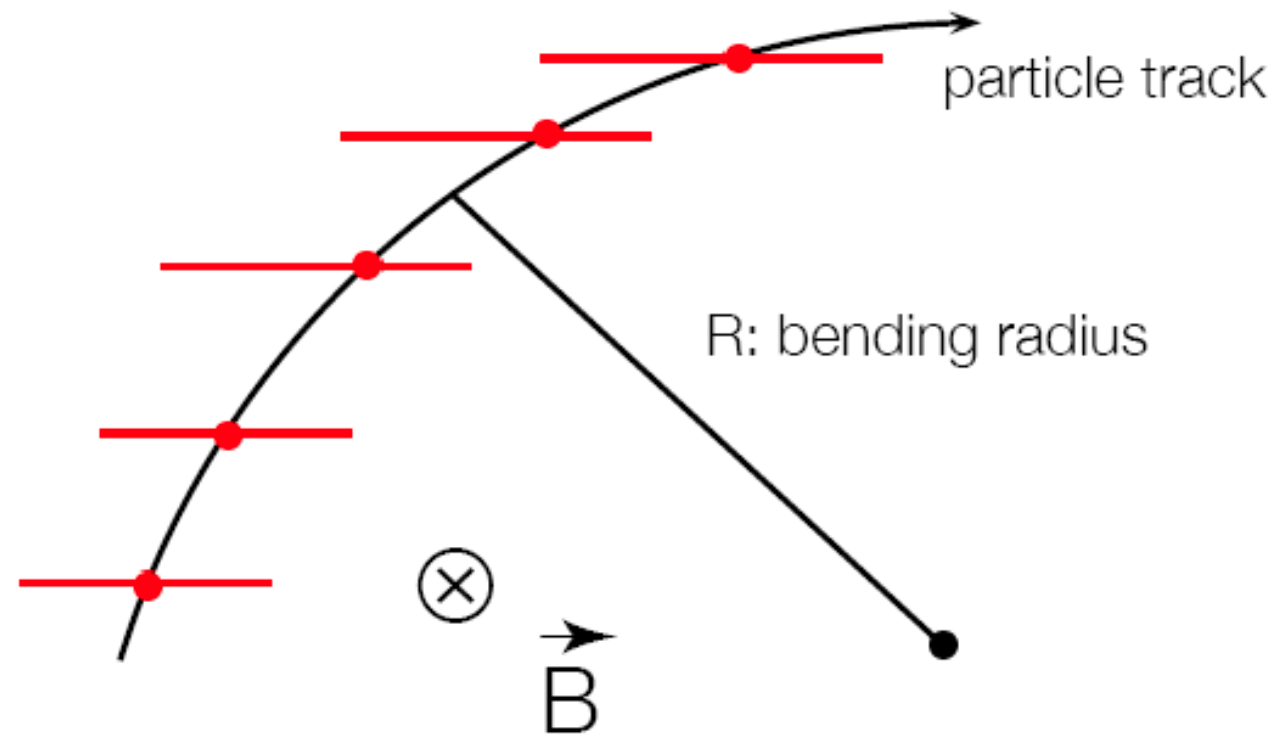
\includegraphics[width=0.75\textwidth]{\figpath/Chapter3/RadiusOfCurvature}
	\caption{Schematic view of a particle track with hits labeled.}
	\label{fig:radius_of_curvature}
\end{figure}

In each subsequent iteration the track seeding criteria is loosened and the same proceedure occurs.
The looser seeding requirments boosts the tracking efficiency, while the removal of the hits from the previous iteration keeps the fake rate low due to the reduced combinatorics.
The specific seeding criteria for each iteration can also be found in table~\ref{tab:track_seeding}.
After three iterations, 90\% of charged hadron tracks within jets are reconstructed and 99.5\% of muons in the tracker acceptance are found.
Subsequent iterations loosen the constraints on the origin vertex, which allows for the reconstructions of tracks associated with a secondary vertex (i.e. $\gamma\rightarrow$\Pep\Pem~conversions, long-lived particles, nuclear interactions in the tracker material).
Tracks meeting this set of criteria can be reconstructed with as little as three hits, a \pt as low as 150\mev, and a vertex  more than 50\unit{cm} away from the beam axis.
Nevertheless, the fake rate is still kept on the order of 1\%~\cite{CMS-PAS-PFT-09-001}.

\begin{table}[htbp]
	\caption{The seed criteria used in each iteration during the 2012 run. The seed types, pair and triplet, indicate if two or three RecHits are used, respectively. The $\sigma$ in the $z_0$ criteria indicated the length of the beam spot in the $z$-direction as determined by a Gaussian fit~\cite{Tracking2012}.}
	\centering
    \begin{tabular}{llllll}
		\hline
		step  & seed type & seed sub-detectors & \pt $[\GeVcns]$ & $d_0$ [cm] & $|z_0|$ \\
		\hline
		0     & triplet   & pixel             & ${>}0.6$     & ${<}0.02$  & ${<}4.0\sigma$ \\
		1     & triplet   & pixel             & ${>}0.2$     & ${<}0.02$  & ${<}4.0\sigma$ \\
		2     & pair      & pixel             & ${>}0.6$     & ${<}0.015$ & ${<}0.09\cm$ \\
		3     & triplet   & pixel             & ${>}0.3$     & ${<}1.5$   & ${<}2.5\sigma$ \\
		4     & triplet   & pixel/TIB/TID/TEC & ${>}0.5$--0.6 & ${<}1.5$   & ${<}10.0\cm$ \\
		5     & pair      & TIB/TID/TEC       & ${>}0.6$     & ${<}2.0$   & ${<}10.0\cm$ \\
		6     & pair      & TOB/TEC           & ${>}0.6$     & ${<}2.0$   & ${<}30.0\cm$ \\
		\hline
    \end{tabular}
	\label{tab:track_seeding}
\end{table}

The tracks found will have a helical shape of with a given radius of curvature as in fig~\ref{fig:radius_of_curvature}.
The softest, low \pt particle trajectories can form small rings, while the higher \pt particles will be bent less.
The momentum of each track can be extracted from the radius of curvature (R), given by a circular fit to the track, the magnetic field strength, as well as $\eta$ and $\varphi$ of the track at the interaction point\footnote{The $\eta$ of the track is determined as if the interaction point was at the center of the detector.}.
The following system of equations can be used to determine the particles 3-momenta at the interaction point:
\begin{equation}
	\begin{aligned}
		p_{x}&=p_{T}\cos\varphi\\
		p_{y}&=p_{T}\sin\varphi\\
		p_{z}&=p_{T}\sinh\eta\\
		p_{T}&=0.3\cdot{B}\cdot{R}
	\end{aligned}
\end{equation}

After the collection of high purity tracks is created, CMS uses these to reconstruct the location of the vertices where proton-proton interactions occurred~\cite{TRK-11-001}.
The vertex finding algorithm is agnostic to whether or not the vertices come from the main hard scatter vertex of interest or any of the pileup vertices from additional proton-proton interactions.
However, there is a need to select prompt tracks occuring near the interaction point instead of tracks from secondary vertices.
CMS requires that the signifigance of the transverse impact parameter $d_{0}<5$, the number of pixel hits be $\geq2$, the number of pixel and stip hits be $\geq5$, and the track $\chi^{2}<20$.
Once there is a collection of prompt tracks they are clustered together in $z$ at their closest approach to the beam spot.
A balance must be struck between vertex finding efficiency and the splitting of good vertices.
To do this, a deterministic annealing (DA) algorithm is used, which is used in cases where one wants to find the approximate global minimum of a problem with many degrees of freedom; specifically where an approximate global minimum is prefered over a more accurate local minimum.
More information about DA can be found in~\cite{Rose1998}, but simply put the process is similar to what happens when one heats a system and then slowly cools it to minimize the ``free energy,'' which in this analogy is the $\chi^{2}$ of the vertices.
In this case there is a system of $z^{T}_{i}$ with uncertainty $\sigma^{z}_{i}$ and an unknown number of vertices $z^{V}_{k}$.
There is a probability $0\leq{p_{ik}}\leq1$ for any track $i$ to be assigned to verted $k$ and in the beginning, the algorithm assumes that every possible assignment is equally likely.
The free energy to be minimized can be found in equation~\ref{eq:DA_free_energy}, where $p_{i}$ is a constant weight for each tracks representing their consitency with originating from the beam spot and $z_{k}^{V}$ are the vertices with weights $\rho_{k}$.
\begin{equation}
	\label{eq:DA_free_energy}
	F=-T\sum_{i}^{\#tracks}p_{i}\log\sum_{k}^{\#vertices}\rho_{k}\exp\left[-\frac{1}{T}\frac{\left(z_{i}^{T}-z_{k}^{V}\right)^{2}}{{\sigma_{i}^{z}}^{2}}\right]
\end{equation}

The number of vertices can be arbitrarily large, but any extra vertices used in the method will overlap with the effective vertices already found at distinct positions.
The probability that a given track corresponds to a specific vertex is given by equation ~\ref{eq:DA_assignment_probability}.
\begin{equation}
	\label{eq:DA_assignment_probability}
	p_{ik}=\frac{\rho_{k}\exp\left[-\frac{1}{T}\frac{\left(z_{i}^{T}-z_{k}^{V}\right)^{2}}{{\sigma_{i}^{z}}^{2}}\right]}{\sum_{k'}\rho_{k'}\exp\left[-\frac{1}{T}\frac{\left(z_{i}^{T}-z_{k'}^{V}\right)^{2}}{{\sigma_{i}^{z}}^{2}}\right]}
\end{equation} 
At high temperature all tracks belong to a single vertex and all $p_{ik}$ are equal.
As $T\rightarrow0$ the each track become compatible with exactly one vetex.
The number of vertices grows each time the temperature falls below the critical temperature of a given vertex, $T_{c}^{k}$, given by equation~\ref{eq:DA_critical_temperature}, where that vertex is replaced by two nearby vertices.
As this happens the tracks are reassigned according to their probabilities before the temperature is lowered again.
The starting temperature of the whole process is chosen to be above the first critical temperature where $\rho_{1}=p_{i1}=1$.
The temperature is lowered by a cooling factor of 0.6 down to $T_{min}=4$, which balances the need to resolve all true vertices with the risk of splitting a true vertex.
\begin{equation}
	\label{eq:DA_critical_temperature}
	T_{c}^{k}=2\sum_{i}\frac{p_{i}p_{ik}}{{\sigma_{i}^{z}}^{2}}\left(\frac{z_{i}^{T}-z_{k}^{V}}{\sigma_{i}^{z}}\right)/\sum_{i}\frac{p_{i}p_{ik}}{{\sigma_{i}^{z}}^{2}}
\end{equation}
By the time the $T_{min}$ condition is reached it is still possible for a track to be assigned to multiple vertices.
Thus, for the final track assignment, the temperature is cooled to $T=1$, without more splitting of the vertices.
For a track to be assigned to a given vertex it must have a minimum probability of $0.5$ and have passed the outlier mitigation criteria.

After all of the candidate vertices are found using the DA method, the candidates with at least two tracks assigned to them are passed through the adaptive vertex fitter (AVF) to compute all of the vertex parameters.
Key among those parameters are the spacial coordinates and the number of degrees of freedom given by equation~\ref{eq:AVF_ndof}, where $w_{i}$ is a weight, between 0 and 1, given to each track depending on the likelihood that the track actually belongs to that vertex.
\begin{equation}
	\label{eq:AVF_ndof}
	n_{dof}=-3+2\sum_{i=1}^{\#tracks}w_{i}
\end{equation}

The methodology above is a simplification of the actual track and vertex finding algorithms, but is sufficiently detailed for the purposes of this document. The subsequent sections will discuss how these most basic detector objects are used to reconstruct particles.

\section{Particle Flow}
\label{sec:particle_flow}

The CMS experiment has decided to use a holistic approach to reconstucting the event produced by a proton-proton collision.
The particle flow (PF) event reconstuction algorithm uses information from all of the sub-detectors in order to reconstruct (direction and energy) and identify as accurately as possible each individual particle in the event as descibed in the first part of this chapter~\cite{CMS-PAS-PFT-09-001}.
The CMS detector, with its extremely granular sub-detectors and high magnetic field, is ideally suited for a particle flow approach.
With the current algorithm, charged-particle tracks out to \absetalt{2.6} can be reconstucted even with a \pt as low as 150\mev, all while maintaining a high reconstruction efficiency and low fake rate.
Photons can be separated from charged-particle energy deposits even in high multiplicity environments like jets.
Although the HCAL is 25 times coarser than the ECAL, the energy resolution is enough to detect neutral hadrons as an energy excess above that deposited by charged hadrons.
Fig~\ref{fig:particle_flow} show, in graphical terms, how the reconstruction algorithm can classify a particle based on the sub-detectors with which it interacts.
The PF algorithm's performance and commisioning is discussed in~\cite{CMS-PAS-PFT-10-002,CMS-PAS-PFT-10-003} using early CMS data and again using newer data and a slightly updated algorithm in~\cite{Beaudette:2014cea}.
All three of these papers indicate a significant improvement in particle identification and object reconstruction over simpler approaches.

The inputs to the PF algorithm come from the local reco products, RecHits, as described at the start of chapter~\ref{ch:event_reconstruction}. More specifically the RecHits are turned into either tracks or energy clusters, which are then used by the algorithm. The tracks may come from the tracker, as described in section~\ref{sec:tracks_and_vertices}, or from the muon system. The clusters are created by the calorimeter RecHits and are treated slightly different than the CaloTowers previously discussed. A local energy maxima









The output of the PF algorithm is a list of particles known as ``PF candidates,'' which are used to build the higher level objects that physicists analyze, such as jets, taus, and \ETmiss. Other quantities that can be determined from a particle level reconstruction algorithm are the charged lepton isolation and the likelihood that a jet was initiated by a B hadron.





\begin{figure}[!hbt]
	\centering
	\begin{subfigure}[t]{0.53\textwidth}
		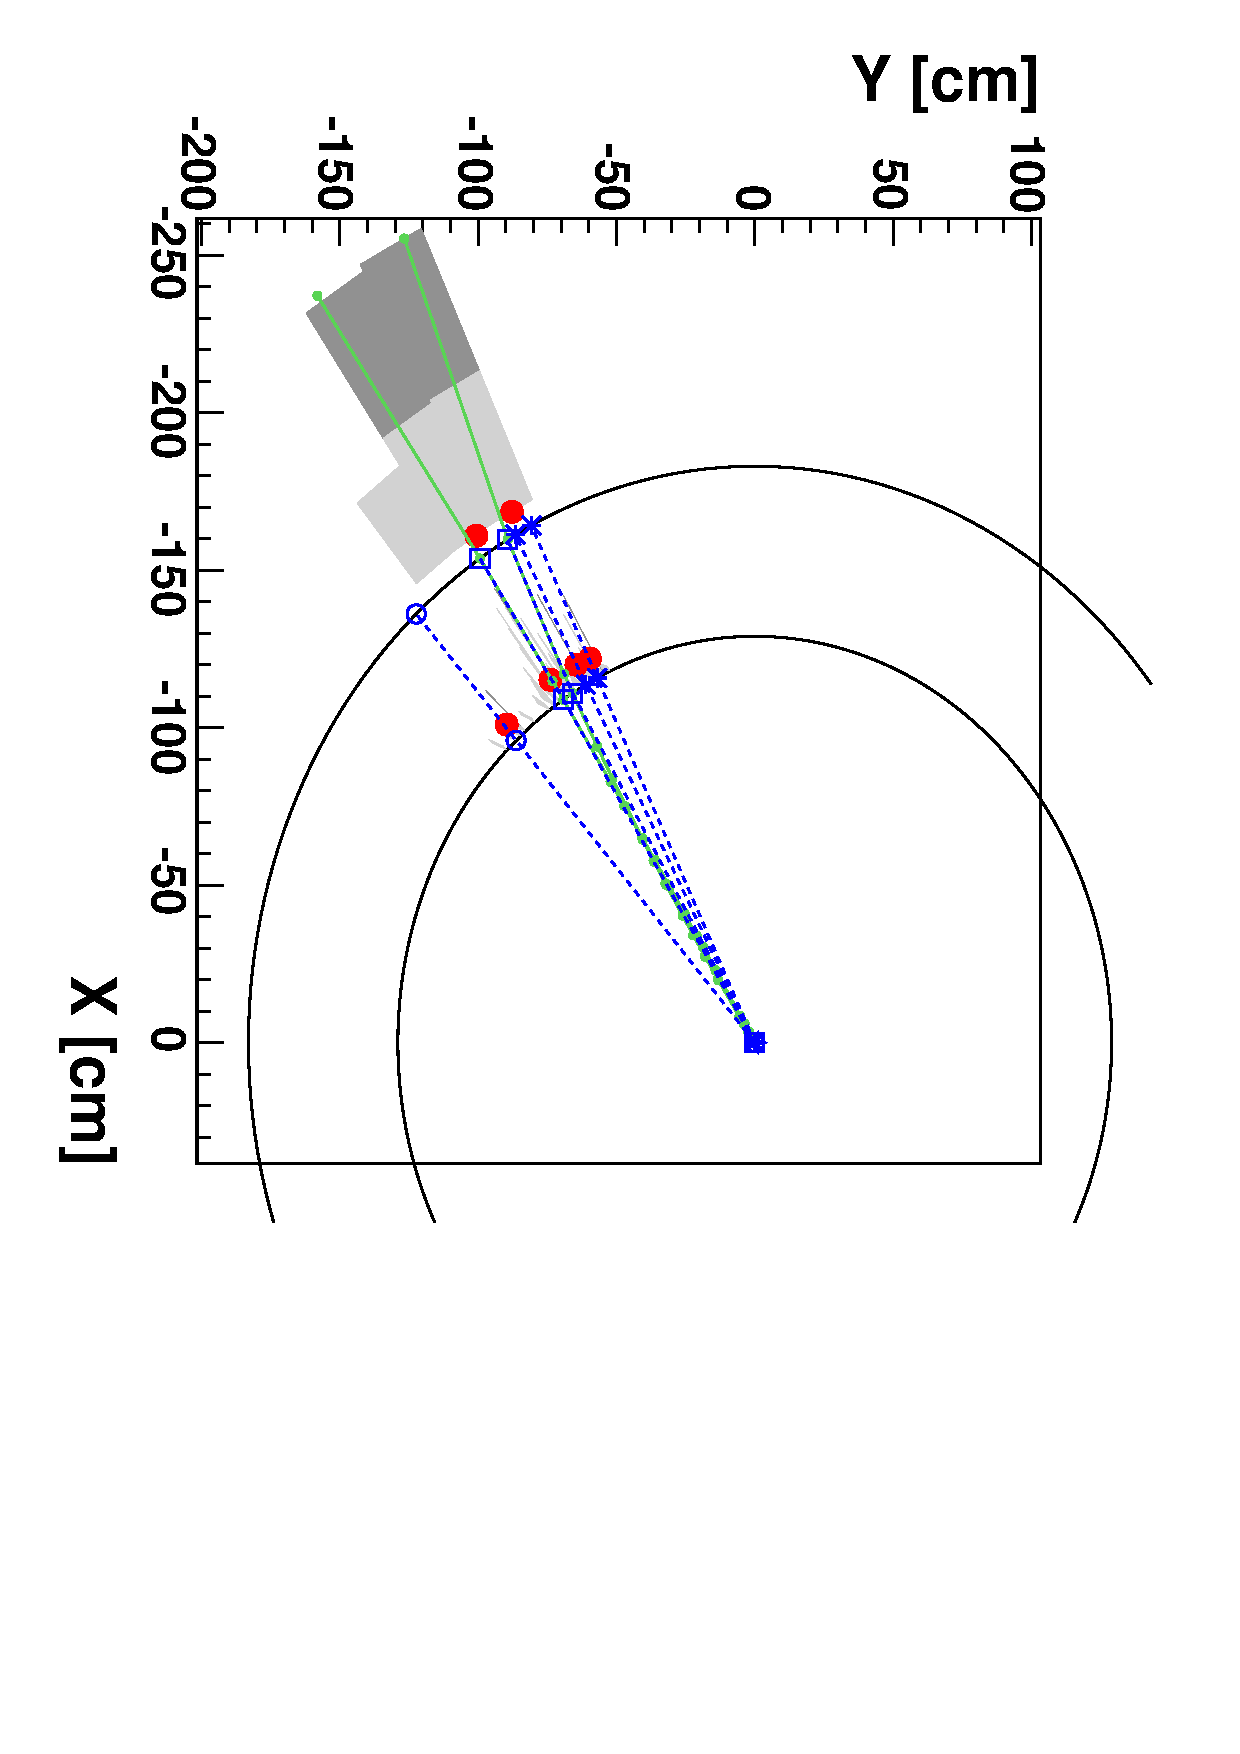
\includegraphics[width=\textwidth,angle=90]{\figpath/Chapter3/PFT-09-001_001_a.pdf}
		\caption{An $(x,y)$ view of the detector.}
		\label{fig:PF_linking_a}
	\end{subfigure}

	\begin{subfigure}[t]{0.4655\textwidth}
		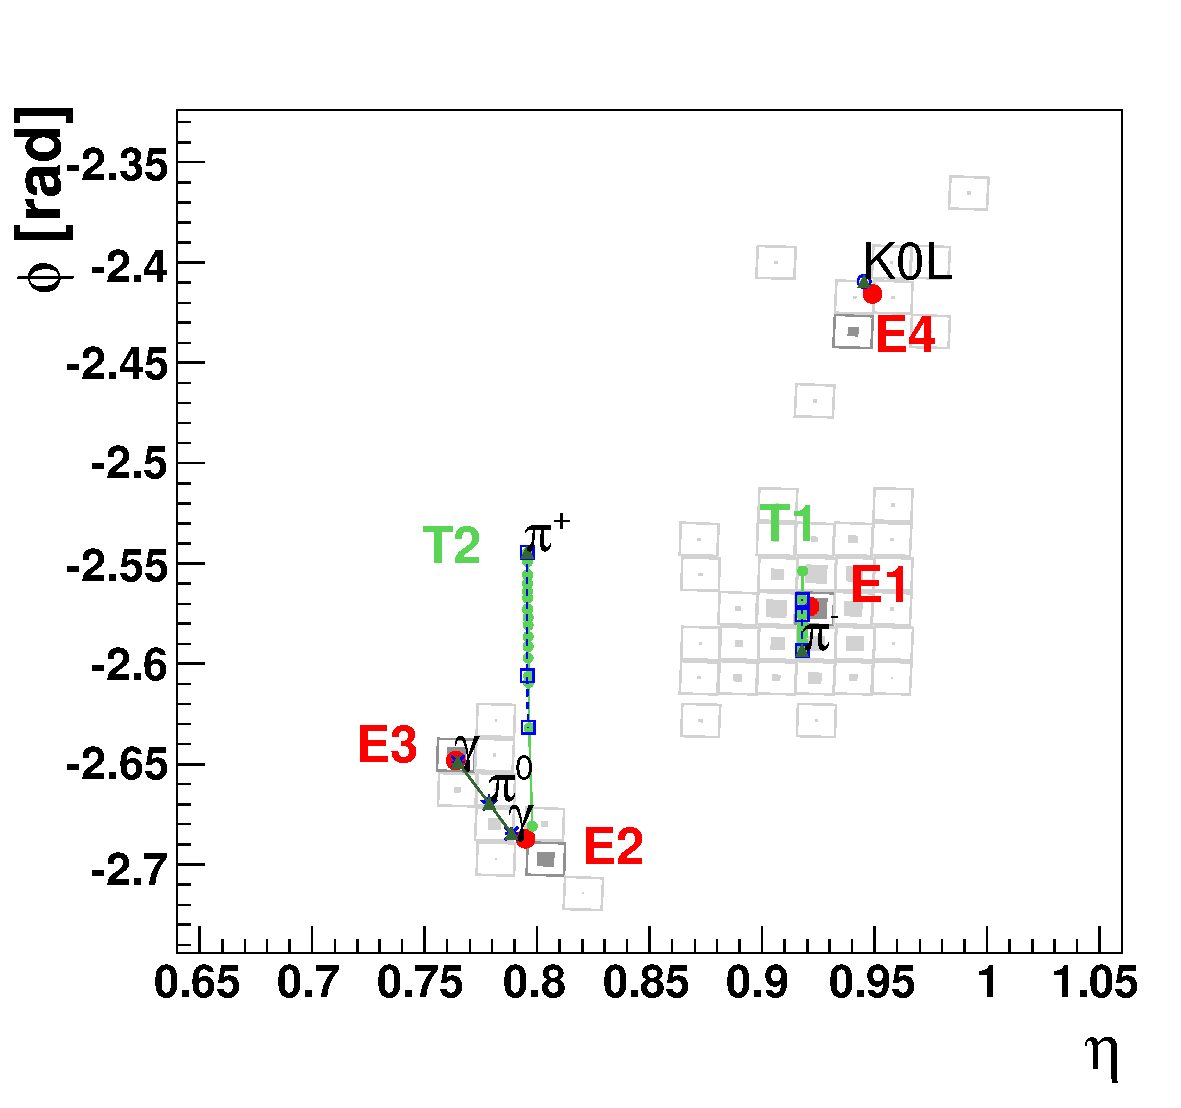
\includegraphics[width=\textwidth]{\figpath/Chapter3/PFT-09-001_001_b.pdf}
		\caption{An $(\eta,\varphi)$ view of the ECAL.}
		\label{fig:PF_linking_b}
	\end{subfigure}
	\begin{subfigure}[t]{0.4655\textwidth}
		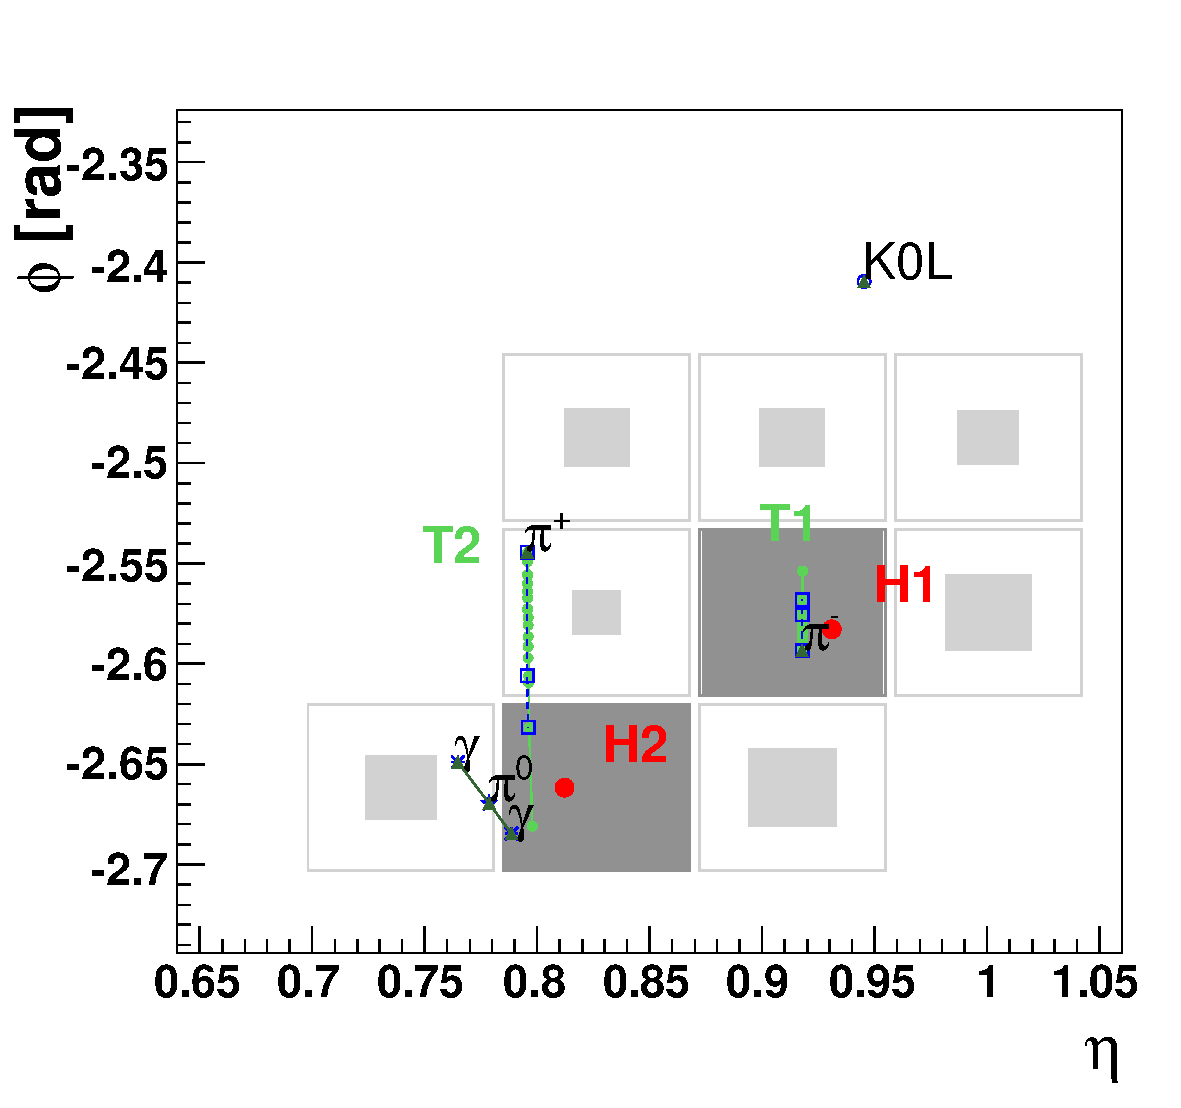
\includegraphics[width=\textwidth]{\figpath/Chapter3/PFT-09-001_001_c.pdf}
		\caption{An $(\eta,\varphi)$ view of the HCAL.}
		\label{fig:PF_linking_c}
	\end{subfigure}
	\caption{These three figures show a representation of how the PF algorithm sees a hadronic jet. (a) An $(x,y)$ view of the detector with elements from the tracker, ECAL, and HCAL shown. The ECAL and HCAL surfaces shown in (b) and (c) are represented by the concentric circles centered around the interaction point in (a). (b) shows the energy clusters from the \PKzL, \Pgpm, and the two photons from the \Pgpz decay. While the \Pgpp doesn't deposit any energy in the ECAL, it does show up as a cluster in the HCAL along with the \Pgpm (c). The tracks from these charged particles show up as vertical lines in the $(\eta,\varphi)$ plane, but as curved lines in the $(x,y)$ plane. The cluster positions are represented by dots, the simulated particles by dashed lines, and the position at which the particles impact the calorimeter surfaces by the open markers~\cite{CMS-PAS-PFT-09-001}.}
\end{figure}

\clearpage











In longer papers, the particle-flow algorithm can be described in more detail:

The global event reconstruction (also called particle-flow event reconstruction~\cite{CMS-PAS-PFT-09-001,CMS-PAS-PFT-10-001}) consists of reconstructing and identifying each individual particle with an optimized combination of all subdetector information.
In this process, the identification of the particle type (photon, electron, muon, charged hadron, neutral hadron) plays an important role in the determination of the particle direction and energy.
Photons (\eg coming from \Pgpz\ decays or from electron bremsstrahlung) are identified as ECAL energy clusters not linked to the extrapolation of any charged particle trajectory to the ECAL.
Electrons (\eg coming from photon conversions in the tracker material or from \cPqb-hadron semileptonic decays) are identified as a primary charged particle track and potentially many ECAL energy clusters corresponding to this track extrapolation to the ECAL and to possible bremsstrahlung photons emitted along the way through the tracker material.
Muons (\eg from \cPqb-hadron semileptonic decays) are identified as a track in the central tracker consistent with either a track or several hits in the muon system, associated with an energy deficit in the calorimeters.
Charged hadrons are identified as charged particle tracks neither identified as electrons, nor as muons.
Finally, neutral hadrons are identified as HCAL energy clusters not linked to any charged hadron trajectory, or as ECAL and HCAL energy excesses with respect to the expected charged hadron energy deposit.

The energy of photons is directly obtained from the ECAL measurement, corrected for zero-suppression effects.
The energy of electrons is determined from a combination of the track momentum at the main interaction vertex, the corresponding ECAL cluster energy, and the energy sum of all bremsstrahlung photons attached to the track.
The energy of muons is obtained from the corresponding track momentum.
The energy of charged hadrons is determined from a combination of the track momentum and the corresponding ECAL and HCAL energy, corrected for zero-suppression effects and for the response function of the calorimeters to hadronic showers.
Finally, the energy of neutral hadrons is obtained from the corresponding corrected ECAL and HCAL energy.


\section{Electrons}

The electron momentum is estimated by combining the energy measurement in the ECAL with the momentum measurement in the tracker.The momentum resolution for electrons with $\pt \approx 45\GeV$ from $\Z \rightarrow \Pe \Pe$ decays ranges from 1.7\% for nonshowering electrons in the barrel region to 4.5\% for showering electrons in the endcaps~\cite{Khachatryan:2015hwa}.

The dielectron mass resolution for $\Z \rightarrow \Pe \Pe$ decays when both electrons are in the ECAL barrel is 1.9\%, and is 2.9\% when both electrons are in the endcaps. The electron momenta are estimated by combining energy measurements in the ECAL with momentum measurements in the tracker~\cite{Khachatryan:2015hwa}. 

\section{Muons}

\section{Jets}
\label{sec:jets}

When combining information from the entire detector, the jet energy resolution amounts typically to 15\% at 10\GeV, 8\% at 100\GeV, and 4\% at 1\TeV, to be compared to about 40\%, 12\%, and 5\% obtained when the ECAL and HCAL calorimeters alone are used.


Traditional calorimetric jets are reconstructed offline from the energy deposits in the calorimeter towers, clustered by the anti-$k_\mathrm{t}$ algorithm~\cite{Cacciari:2008gp, Cacciari:2011ma} with a size parameter of 0.4. In this process, the contribution from each calorimeter tower is assigned a momentum, the absolute value and the direction of which are given by the energy measured in the tower, and the coordinates of the tower. The raw jet energy is obtained from the sum of the tower energies, and the raw jet momentum by the vectorial sum of the tower momenta, which results in a nonzero jet mass. The raw jet energies are then corrected to establish a relative uniform response of the calorimeter in $\eta$ and a calibrated absolute response in transverse momentum \pt. 

 The particle-flow algorithm can be described in short form as:

The particle-flow event algorithm reconstructs and identifies each individual particle with an optimized combination of information from the various elements of the CMS detector. The energy of photons is directly obtained from the ECAL measurement, corrected for zero-suppression effects. The energy of electrons is determined from a combination of the electron momentum at the primary interaction vertex as determined by the tracker, the energy of the corresponding ECAL cluster, and the energy sum of all bremsstrahlung photons spatially compatible with originating from the electron track. The energy of muons is obtained from the curvature of the corresponding track. The energy of charged hadrons is determined from a combination of their momentum measured in the tracker and the matching ECAL and HCAL energy deposits, corrected for zero-suppression effects and for the response function of the calorimeters to hadronic showers. Finally, the energy of neutral hadrons is obtained from the corresponding corrected ECAL and HCAL energy.

to be followed by these other lines, after mentioning the anti-\kt algorithm:

Jet momentum is determined as the vectorial sum of all particle momenta in the jet, and is found from simulation to be within 5 to 10\% of the true momentum over the whole \pt spectrum and detector acceptance. An offset correction is applied to jet energies to take into account the contribution from additional proton-proton interactions within the same or nearby bunch crossings. Jet energy corrections are derived from simulation, and are confirmed with in situ measurements of the energy balance in dijet and photon + jet events. Additional selection criteria are applied to each event to remove spurious jet-like features originating from isolated noise patterns in certain HCAL regions.

In some papers, you would want to add some performance numbers:

The jet energy resolution amounts typically to 15\% at 10\GeV, 8\% at 100\GeV, and 4\% at 1\TeV, to be compared to about 40\%, 12\%, and 5\% obtained when the calorimeters alone are used for jet clustering.

For each event, hadronic jets are clustered from these reconstructed particles with the infrared and collinear safe anti-\kt algorithm, operated with a size parameter $R$ of 0.4. The jet momentum is determined as the vectorial sum of all particle momenta in this jet, and is found in the simulation to be within 5 to 10\% of the true momentum over the whole \pt spectrum and detector acceptance. Jet energy corrections are derived from the simulation, and are confirmed with in situ measurements with the energy balance of dijet and photon + jet events~\cite{Chatrchyan:2011ds}. The jet energy resolution amounts typically to 15\% at 10\GeV, 8\% at 100\GeV, and 4\% at 1\TeV, to be compared to about 40\%, 12\%, and 5\% obtained when the calorimeters alone are used for jet clustering. 

\section{Missing Transverse Energy}


\section{Event Generation}

\section{Detector Simulation}